\documentclass[tikz,border=10pt]{standalone}
\usetikzlibrary{shapes}
\usepackage{calc}

\newcommand{\level}{11}
\newcommand{\ybound}{3}

\begin{document}
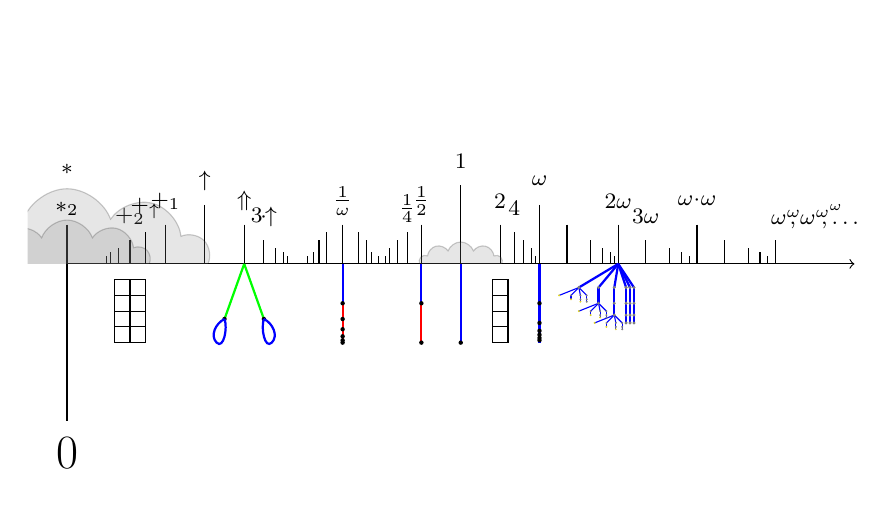
\begin{tikzpicture}[font=\LARGE] 
\node (z) at (0,0) {};
\node (e) at (10,0) {};
\draw [->] (z.center) -- (e.center);

\draw[color=black] (0pt, 0.5) -- (0pt, -2);
\node at (0, -2.4) {0};

// Set Bounds
\begin{scope}
	\clip (-0.5, -\ybound) rectangle (\ybound, \ybound);
\end{scope}

\ifnum\level>0
\foreach \x/\lab/\size in {5/1/1,5.5/2/0.5, 5.68/4/0.4, 5.8/ /0.3, 5.9/ /0.2, 5.95/ /0.1} {
\draw (\x, \size) -- (\x, 0);
\node at (\x, \fpeval{0.3+\size}) {\footnotesize \lab};
}
\fi

\ifnum\level>1
\foreach \x/\lab/\size in {4.5/$\frac{1}{2}$/0.5, 4.32/$\frac{1}{4}$/0.4, 4.2/ /0.3, 4.1/ /0.2, 4.05/ /0.1} {
\draw (\x, \size) -- (\x, 0);
\node at (\x, \fpeval{0.3+\size}) {\footnotesize \lab};
}
\fi

\ifnum\level>2
\draw (3.5, 0.5) -- (3.5, 0);
\node at (3.5, \fpeval{0.8}) {\footnotesize $\frac{1}{\omega}$};
\foreach \x/\lab/\size in {3.05/ /0.1, 3.13/ /0.15, 3.2/ /0.3, 3.3/$\frac{1}{2\omega}$/0.4,3.7/$\frac{2}{\omega}$/0.4, 3.8/ /0.3, 3.87/ /0.15, 3.95/ /0.1} {
\draw (\x, \size) -- (\x, 0);
}
\fi

\ifnum\level>3
\draw (1.75, 0.75) -- (1.75, 0);
\node at (1.75, \fpeval{1.05}) {\footnotesize $\uparrow$};
% \node at (1.75, \fpeval{-1.05}) {\footnotesize $+_{0}$};
\foreach \x/\lab/\size in {2.25/$\Uparrow$/0.5, 2.5/$3\hspace{-0.1em}\cdot\hspace{-0.35em}\uparrow$/0.3, 2.65/ /0.2, 2.75/ /0.15, 2.8/ /0.1} {
\draw (\x, \size) -- (\x, 0);
\node at (\x, \fpeval{0.3+\size}) {\footnotesize \lab};
}
\fi

\ifnum\level>4
\draw (6, 0.75) -- (6, 0);
\node at (6, \fpeval{1.05}) {\footnotesize $\omega$};
\foreach \x/\lab/\size in {6.35/$\omega\hspace{-0.2em}+\hspace{-0.2em}1$/0.5, 6.65/$\omega\hspace{-0.2em}+\hspace{-0.2em}2$/0.3, 6.8/ /0.2, 6.9/ /0.15, 6.95/ /0.1} {
\draw (\x, \size) -- (\x, 0);
}
\fi

\ifnum\level>5
\draw (7, 0.5) -- (7, 0);
\node at (7, \fpeval{0.8}) {\footnotesize $2\omega$};
\draw (8, 0.5) -- (8, 0);
\node at (8, \fpeval{0.8}) {\footnotesize $\omega\hspace{-0.2em}\cdot\hspace{-0.2em}\omega$};
\foreach \x/\lab/\size in {7.35/$3\omega$/0.3, 7.65/ /0.2, 7.8/ /0.15, 7.9/ /0.1, 8.35/ /0.3, 8.65/ /0.2, 8.8/ /0.15, 8.9/ /0.1} {
\draw (\x, \size) -- (\x, 0);
\node at (\x, \fpeval{0.3+\size}) {\footnotesize \lab};
}
\fi

\ifnum\level>6
\draw (9, 0.3) -- (9, 0);
\node at (9.5, \fpeval{0.6}) {\footnotesize $\omega^\omega\hspace{-0.5em},\omega^{\omega^\omega}\hspace{-1.0em},\ldots$};
\fi

\ifnum\level>7
\foreach \x/\lab/\size in {1.25/$+_1$/0.5, 0.8/$+_2$/0.3, 0.65/ /0.2, 0.55/ /0.15, 0.5/ /0.1} {
\draw (\x, \size) -- (\x, 0);
\node at (\x, \fpeval{0.3+\size}) {\footnotesize \lab};
}
\fi


\ifnum\level>8

\node at (0, 1.2) {\footnotesize $*$};

\begin{scope}
	\clip (-0.5, 0) rectangle (\ybound, \fpeval{\ybound / 2});
	\node[cloud, draw, cloud puffs=10, cloud puff arc=140, aspect=3, inner ysep=1.2em, fill=gray, opacity=0.2] {};
\end{scope}
\fi

\ifnum\level>9
\draw (1, 0.4) -- (1, 0);

\node at (0, 0.7) {\footnotesize $*_2$};
\node at (1, 0.7) {\footnotesize $+_{\uparrow}$};

\begin{scope}
	\clip (-0.5, 0) rectangle (\ybound, \fpeval{\ybound / 2});
	\node[cloud, draw, cloud puffs=10, cloud puff arc=140, aspect=3, inner ysep=0.7em, fill=gray, opacity=0.2] {};
\end{scope}
\fi

\ifnum\level>10
\begin{scope}
	\clip (-0.5, 0) rectangle (10, \fpeval{\ybound / 2});
	\node[cloud, draw, cloud puffs=10, cloud puff arc=140, aspect=3, inner ysep=0.35em, fill=gray, opacity=0.2] at (5, 0) {};
\end{scope}
\fi

\draw [blue, thick] (5,0) -- (5,-1);
\fill (5, -1) circle[radius=0.8pt];


\draw [blue, thick] (4.5,0) -- (4.5,-0.5);
\draw [red, thick] (4.5,-0.5) -- (4.5,-1);
\fill (4.5, -0.5) circle[radius=0.8pt];
\fill (4.5, -1) circle[radius=0.8pt];

\draw [blue, thick] (3.5,0) -- (3.5,-0.5);
\draw [red, thick] (3.5,-0.5) -- (3.5,-1);
\fill (3.5, -0.5) circle[radius=0.8pt];
\fill (3.5, -0.7) circle[radius=0.8pt];
\fill (3.5, -0.83) circle[radius=0.8pt];
\fill (3.5, -0.92) circle[radius=0.8pt];
\fill (3.5, -0.97) circle[radius=0.8pt];
\fill (3.5, -1) circle[radius=0.8pt];

\draw (5.4, -0.2) -- (5.6, -0.2) -- (5.6, -1) -- (5.4, -1) -- (5.4, -0.2);
\draw (5.4, -0.4) -- (5.6, -0.4);
\draw (5.4, -0.6) -- (5.6, -0.6);
\draw (5.4, -0.8) -- (5.6, -0.8);

\draw [blue, thick] (6,0) -- (6,-1);
\fill (6, -0.5) circle[radius=0.8pt];
\fill (6, -0.75) circle[radius=0.8pt];
\fill (6, -0.85) circle[radius=0.8pt];
\fill (6, -0.9) circle[radius=0.8pt];
\fill (6, -0.94) circle[radius=0.8pt];
\fill (6, -0.97) circle[radius=0.8pt];

\draw [green, thick] (2.25, 0) -- (2, -0.7);
\draw [green, thick] (2.25, 0) -- (2.5, -0.7);
\fill (2, -0.7) circle[radius=0.8pt];
\fill (2.5, -0.7) circle[radius=0.8pt];
\draw [blue, thick] (2.5, -0.7) to[out=-25,in=45] (2.6, -1) to[in=-110, out=225] (2.5, -0.7);
\draw [blue, thick] (2, -0.7) to[out=205,in=135] (1.9, -1) to[in=290, out=-45] (2, -0.7);

\draw (0.8, -0.2) -- (0.6, -0.2) -- (0.6, -1) -- (0.8, -1) -- (0.8, -0.2);
\draw (0.8, -0.4) -- (0.6, -0.4);
\draw (0.8, -0.6) -- (0.6, -0.6);
\draw (0.8, -0.8) -- (0.6, -0.8);
\draw (0.8, -0.2) -- (1, -0.2) -- (1, -1) -- (0.8, -1) -- (0.8, -0.2);
\draw (0.8, -0.4) -- (1, -0.4);
\draw (0.8, -0.6) -- (1, -0.6);
\draw (0.8, -0.8) -- (1, -0.8);

\draw[blue] (6.5, -0.3) -- (6.25, -0.4);
\draw[blue] (6.5, -0.3) -- (6.4, -0.4);
\draw[blue] (6.5, -0.3) -- (6.52, -0.4);
\draw[blue] (6.5, -0.3) -- (6.6, -0.4);
\draw[blue] (6.4, -0.4) -- (6.4, -0.45);
\draw[blue] (6.52, -0.4) -- (6.52, -0.45);
\draw[blue] (6.6, -0.4) -- (6.6, -0.45);
\draw[blue] (6.52, -0.48) -- (6.52, -0.45);
\draw[blue] (6.6, -0.48) -- (6.6, -0.45);

\draw[blue] (6.75, -0.5) -- (6.5, -0.6);
\draw[blue] (6.75, -0.5) -- (6.65, -0.6);
\draw[blue] (6.75, -0.5) -- (6.77, -0.6);
\draw[blue] (6.75, -0.5) -- (6.85, -0.6);
\draw[blue] (6.65, -0.6) -- (6.65, -0.65);
\draw[blue] (6.77, -0.6) -- (6.77, -0.65);
\draw[blue] (6.85, -0.6) -- (6.85, -0.65);
\draw[blue] (6.77, -0.68) -- (6.77, -0.65);
\draw[blue] (6.85, -0.68) -- (6.85, -0.65);

\draw[blue] (6.95, -0.65) -- (6.7, -0.75);
\draw[blue] (6.95, -0.65) -- (6.85, -0.75);
\draw[blue] (6.95, -0.65) -- (6.97, -0.75);
\draw[blue] (6.95, -0.65) -- (7.05, -0.75);
\draw[blue] (6.85, -0.75) -- (6.85, -0.8);
\draw[blue] (6.97, -0.75) -- (6.97, -0.8);
\draw[blue] (7.05, -0.75) -- (7.05, -0.8);
\draw[blue] (6.97, -0.83) -- (6.97, -0.8);
\draw[blue] (7.05, -0.83) -- (7.05, -0.8);

\draw[blue, thick] (7, 0) -- (6.5, -0.3);
\draw[blue, thick] (7, 0) -- (6.75, -0.3);
\draw[blue, thick] (7, 0) -- (6.95, -0.3);
\draw[blue, thick] (7, 0) -- (7.1, -0.3);
\draw[blue, thick] (7, 0) -- (7.15, -0.3);
\draw[blue, thick] (7, 0) -- (7.2, -0.3);

\draw[blue, thick] (6.75, -0.3) -- (6.75, -0.5);
\draw[blue, thick] (6.95, -0.3) -- (6.95, -0.5);
\draw[blue, thick] (7.1, -0.3) -- (7.1, -0.5);
\draw[blue, thick] (7.15, -0.3) -- (7.15, -0.5);
\draw[blue, thick] (7.2, -0.3) -- (7.2, -0.5);

\draw[blue, thick] (6.95, -0.65) -- (6.95, -0.5);
\draw[blue, thick] (7.1, -0.65) -- (7.1, -0.5);
\draw[blue, thick] (7.15, -0.65) -- (7.15, -0.5);
\draw[blue, thick] (7.2, -0.65) -- (7.2, -0.5);

\draw[blue, thick] (7.1, -0.65) -- (7.1, -0.75);
\draw[blue, thick] (7.15, -0.65) -- (7.15, -0.75);
\draw[blue, thick] (7.2, -0.65) -- (7.2, -0.75);

\fill[gray] (6.5, -0.3) circle[radius=0.6pt];
\fill[gray] (6.75, -0.3) circle[radius=0.6pt];
\fill[gray] (6.95, -0.3) circle[radius=0.6pt];
\fill[gray] (7.1, -0.3) circle[radius=0.6pt];
\fill[gray] (7.15, -0.3) circle[radius=0.6pt];
\fill[gray] (7.2, -0.3) circle[radius=0.6pt];

\fill[gray] (6.75, -0.5) circle[radius=0.6pt];
\fill[gray] (6.95, -0.5) circle[radius=0.6pt];
\fill[gray] (7.1, -0.5) circle[radius=0.6pt];
\fill[gray] (7.15, -0.5) circle[radius=0.6pt];
\fill[gray] (7.2, -0.5) circle[radius=0.6pt];

\fill[gray] (6.95, -0.65) circle[radius=0.6pt];
\fill[gray] (7.1, -0.65) circle[radius=0.6pt];
\fill[gray] (7.15, -0.65) circle[radius=0.6pt];
\fill[gray] (7.2, -0.65) circle[radius=0.6pt];

\fill[gray] (7.1, -0.75) circle[radius=0.6pt];
\fill[gray] (7.15, -0.75) circle[radius=0.6pt];
\fill[gray] (7.2, -0.75) circle[radius=0.6pt];

\fill[black!15!yellow] (6.25, -0.4) circle[radius=0.4pt];
\fill[gray] (6.4, -0.4) circle[radius=0.4pt];
\fill[gray] (6.52, -0.4) circle[radius=0.4pt];
\fill[gray] (6.6, -0.4) circle[radius=0.4pt];

\fill[black!15!yellow] (6.4, -0.45) circle[radius=0.4pt];
\fill[gray] (6.52, -0.45) circle[radius=0.4pt];
\fill[gray] (6.6, -0.45) circle[radius=0.4pt];

\fill[black!15!yellow] (6.52, -0.48) circle[radius=0.4pt];
\fill[gray] (6.6, -0.48) circle[radius=0.4pt];

\fill[black!15!yellow] (6.5, -0.6) circle[radius=0.4pt];
\fill[gray] (6.65, -0.6) circle[radius=0.4pt];
\fill[gray] (6.77, -0.6) circle[radius=0.4pt];
\fill[gray] (6.85, -0.6) circle[radius=0.4pt];

\fill[black!15!yellow] (6.65, -0.65) circle[radius=0.4pt];
\fill[gray] (6.77, -0.65) circle[radius=0.4pt];
\fill[gray] (6.85, -0.65) circle[radius=0.4pt];

\fill[black!15!yellow] (6.77, -0.68) circle[radius=0.4pt];
\fill[gray] (6.85, -0.68) circle[radius=0.4pt];

\fill[black!15!yellow] (6.7, -0.75) circle[radius=0.4pt];
\fill[gray] (6.85, -0.75) circle[radius=0.4pt];
\fill[gray] (6.97, -0.75) circle[radius=0.4pt];
\fill[gray] (7.05, -0.75) circle[radius=0.4pt];

\fill[black!15!yellow] (6.85, -0.8) circle[radius=0.4pt];
\fill[gray] (6.97, -0.8) circle[radius=0.4pt];
\fill[gray] (7.05, -0.8) circle[radius=0.4pt];

\fill[black!15!yellow] (6.97, -0.83) circle[radius=0.4pt];
\fill[gray] (7.05, -0.83) circle[radius=0.4pt];

\end{tikzpicture}
\end{document}